\chapter{Implementation}\label{chap:Implementation}
This section details the slicing theories developed and implementations of type slicing, cast slicing, and the search procedure.

\section{Type Slicing Theory}\label{sec:TypeSlicingTheory}
I develop a novel method, \textit{type slicing}, to aid programmers in understanding \textit{how} a bidirectional type system works. First I define typing slices. Then, three slicing criteria: synthesis, analysis, and contribution slices, each associate typing derivations with different explanatory slices. 

The first two criteria give insight on the synthesised and analysed type contributions. The third completes a picture of code regions contributing in any way to a term's type.

The second and third criterion were \textit{very challenging} to formalise, requiring non-obvious mathematical machinery: \textit{context typing slices} (\cref{sec:ContextTypingSlices}), \textit{checking contexts} (\cref{sec:CheckingContexts}), and \textit{type-indexed slices} (\cref{sec:TypeIndexedSlices}). Only the basic definitions are given here, the full theory is found in \cref{sec:SlicingTheory}.

\subsection{Expression Typing Slices}\label{sec:ExpressionTypingSlices}
First, I introduce what \textit{slices} are in this context. The aim is to provide a formal representation of term \textit{highlighting}. 

\subsubsection{Term Slices}
A \textit{term slice} is a term with some sub-terms omitted. The omitted terms are those that are \textit{not} highlighted. For example if my slicing criterion is to \textit{omit terms which are typed as} \code{Int}, then the following expressions highlights as:

\[\hlcmaths[yellow!30]{(\lambda} x: \code{Int}\hlcmaths[yellow!30]{.\ \lambda y : \code{Bool}.}\ x\hlcmaths[yellow!30]{)(}1\hlcmaths[yellow!30]{)}\]


Omitted sub-terms are replaced by a \textit{gap} term, notated $\gap$. Representing the example above, we get:
\[(\lambda \gap.\ \lambda y : \code{Bool}.\ \gap)(\gap)\]

We can then define a \textit{precision} partial order \cite{PartialOrder} on term slices: $\varsigma_1 \sqsubseteq \varsigma_2$ meaning $\varsigma_1$ is less or equally precise than $\varsigma_2$. That is, $\varsigma_1$ matches $\varsigma_2$ structurally except that some sub-terms may be gaps. For example:
\[\gap \sqsubseteq\gap + \gap\sqsubseteq 1 + \gap \sqsubseteq 1 + 2\]

\paragraph{Lattice Structure}\label{sec:JoinTypesTheory} For any \textit{complete term} $t$ (having no gaps), the slices of $t$ form a \textit{bounded lattice structure} \cite{Lattice}. That is, every pair $\varsigma_1, \varsigma_2$ has a \textit{join} $\varsigma_1 \sqcup \varsigma_2$ and \textit{meet} $\varsigma_1 \sqcap \varsigma_2$. In general, not all slices slices have joins: $1 \centernot\sqcup\ 2$, but do have meets as $\gap \sqsubseteq \varsigma$ for all $\varsigma$.
 
\subsubsection{Typing Assumption Slices}
Expression typing is performed given a set of \textit{typing assumptions}. Therefore, in addition, we also desire a slice taking the \textit{relevant} assumptions. Typing assumptions are \textit{partial functions} mapping variables to types (see \cref{sec:TypingJudgements}). 

Hence, their slices slices are partial functions to \textit{type slices}. Such that, a slice maps no more variables to no more precise types. This, and meets and joins, can be extended by extensionality \cite{Extensionality}:

\begin{definition}[Typing Assumption Slice Precision]
For typing assumption slices $\gamma_1, \gamma_2$. Where $\mathrm{dom}(f)$ is the set of variables for which a partial function $f$ is \textit{defined}:
\[\gamma_1 \sqsubseteq \gamma_2 \iff \mathrm{dom}(\gamma_1) \subseteq \mathrm{dom}(\gamma_2) \text{ and } \forall x \in  \mathrm{dom}(\gamma_1).\ \gamma_1(x) \sqsubseteq \gamma_2(x)\]
\end{definition}
\begin{definition}[Typing Assumption Slice Joins and Meets]
For typing slices $\gamma_1, \gamma_2$, and any variable $x$: 

If $\gamma_1(x) = \bot$ then $(\gamma_1 \sqcup \gamma_2)(x) = \gamma_2(x)$ and $(\gamma_1 \sqcap \gamma_2)(x) = \bot$, analogously if $\gamma_2(x) = \bot$. Otherwise, $(\gamma_1 \sqcup \gamma_2)(x) = \gamma_1(x) \sqcup \gamma_2(x)$.
\end{definition}
Again, slicing complete typing assumptions $\Gamma$ forms a bounded lattice. In general, some slices have no join: consider $x : \code{Int}$ and $x : \code{String}$.

\subsubsection{Expression Typing Slices}
Finally, an \textit{expression typing slice}, $\rho$, is a pair, $\varsigma^\gamma$, of a term slice and a typing slice. Precision, joins and meets, can be extended pointwise to term typing slices with all the same properties.

\paragraph{Typing Checking} \textit{Expression slices} can be \textit{type checked} under the \textit{type assumption slices} by replacing gaps $\gap$ by: holes of arbitrary metavariable $\hole^u$ in \textit{expressions}, fresh variables in \textit{patterns}, and the dynamic type in \textit{types}. Notated by $\type{\cdot}$.

\begin{definition}[Expression Typing Slice Type Checking]
For expression typing slice $\varsigma^{\gamma}$ and type $\tau$. $\synthesis[\gamma]{\varsigma}{\tau}$ iff $\synthesis[\type{\gamma}]{\type{\varsigma}}{\tau}$ and $\analysis[\gamma]{\varsigma}{\tau}$ iff $\analysis[\type{\gamma}]{\type{\varsigma}}{\tau}$.
\end{definition}
\subsection{Context Typing Slices}\label{sec:ContextTypingSlices}
Next, some of an expression's type might be enforced by the surrounding \textit{context}. For example, the  type of the underlined expression below is enforced by the surrounding highlighted annotation:
\[\underline{(\lambda x. \hole^u )} \hlcmaths[yellow!30]{:  \code{Bool} \hlcmaths[yellow!30]{\to \code{Int}}}\]

\subsubsection{Contexts and Their Slices}
\renewcommand{\C}{\mathdcal{C}}
We represent these surrounding contexts by a \textit{term context} $\mathdcal{C}$. Which marks \textit{exactly one} sub-term as $\cmark$. Where $\C\{t\}$ substitutes term $t$ for the mark $\cmark$ in $\C$, only allowed if the marked position expects a term of the same class as $t$ (pattern \code{Pat}, type \code{Typ}, or expression \code{Exp}). Notate the classes by $\C : \code{X} \to \code{Y}$. Contexts are \textit{composable}: $(\C_1 \circ \C_2)(t) = \C_1\{\C_2\{t\}\}$ when $\C_1 : \code{X} \to \code{Y}$ and $\C_2 : \code{Y} \to \code{Z}$. Composition is associative.


\newcommand{\Cs}{\mathdcal{c}}
\newcommand{\p}{\mathdcal{p}}
These extend to slices analogously to term slices. However, the precision relation $\sqsubseteq$ more restrictive, requiring the mark $\cmark$ to remain in the same structural position. For example: $\cmark(\gap) \sqsubseteq \cmark(1)$, but $\cmark \not \sqsubseteq \cmark(1)$. Concisely defined by \textit{extensionality}:

\begin{definition}[Context Precision]\label{def:ContextPrecision}
If $\Cs : \code{X} \to \code{Y}$ and $\Cs' : \code{X} \to \code{Y}$ are context slices, then $\Cs' \sqsubseteq \Cs$ if and only if, for all terms $t$ of class $\code{X}$, that $\Cs'\{t\} \sqsubseteq \Cs\{t\}$.
\end{definition}

We find that filling contexts preserves the precision relations both on term slices \textit{and} context slices:
\begin{proposition}[Context Filling Preserves Precision]
For context slice $\Cs : \code{X} \to \code{Y}$ and term slice $\varsigma$ of class \code{X}. Then if we have slices $\varsigma' \sqsubseteq \varsigma$, $\Cs' \sqsubseteq \Cs$ then also $\Cs'\{\varsigma'\} \sqsubseteq \Cs\{\varsigma\}$.
\end{proposition}

Joins and meets can be defined extensionally as before, still forming bounded lattices over complete contexts. The lattice bottom is the \textit{purely structural context}, consisting of only gaps with the mark in the correct position. In general, in addition to joins, not all contexts have meets: $\cmark\centernot \sqcap \cmark(\gap)$.

\subsubsection{Typing Assumption Contexts and Their Slices}
The accompanying notion typing notion can be represented by \textit{endomorphisms on typing assumption slices}. These functions represents which \textit{relevant} typing assumptions must be \textit{added}, and those safely \textit{removable} when typing an expression within a context slice.

\renewcommand{\F}{\mathdcal{F}}
\newcommand{\f}{\mathdcal{f}}

Precision, joins, and meets can be defined via extensionality. As usual forming bounded lattices on complete functions, the bottom being the constant function to the empty typing assumptions. Again, such functions are monotone:
\begin{proposition}[Function Application Preserves Precision]
For typing assumption slice $\gamma$ and typing assumption context slice $\f$. Then if we have slices $\gamma' \sqsubseteq \gamma$, $f' \sqsubseteq f$ then also $f'(\gamma') \sqsubseteq f(\gamma)$.
\end{proposition}
\subsubsection{Context Typing Slices}
Finally, an \textit{expression context typing slice}, $\p$, is a pair, $\Cs^\f$, of an expression context slice and a typing assumption context slice defined pointwise, with all the same properties (including composition).

\paragraph{Type Checking} An analogous $\type{\cdot}$ translation can be defined.

\subsection{Type-Indexed Slices}\label{sec:TypeIndexedSlices}
Decomposing slices by their type is required for cast slicing and useful in calculating slices according to analysis slices and hence also contribution slices. For example consider the following context slice explaining why the underlined term analyses $\code{Bool} \to \code{Int}$:
\[\underline{(\lambda x. \hole^u )} \hlcmaths[yellow!30]{:  \code{Bool} \hlcmaths[yellow!30]{\to \code{Int}}}\]
This would be tagged with the type $\code{Bool} \to \code{Int}$ where a sub-slice considering \textit{only} the \code{Int} return type (omitting the \code{Bool} annotation) can be extracted:
\[\underline{(\lambda x. \hole^u )} \hlcmaths[yellow!30]{:}  \code{Bool} \hlcmaths[yellow!30]{\to \code{Int}}\]
This section will only consider \textit{context slices}, but term slices are type-indexed analogously.

The main property that indexed-slices should maintain is that slices can be \textit{reconstructed} from their sub-parts. Joining the sub-slices will produce the full type. As sub-slices may slice different regions of code, we pair them with contexts which place the sub-slices within the same context, making them join-able.

\renewcommand{\S}{\mathdcal{S}}
\renewcommand{\s}{\mathdcal{s}}
\begin{definition}[Type-Indexed Context Typing Slices]
Syntactically defined: 
\[\S ::= \p \mid \p * \S \to \p * \S\] 
With any $\S$ only being valid if it has a full slice. The full slice of $\S$, notated $\overline{\S}$, is defined:
\[\overline{\p} = \p\]
\[\overline{\p_1 * \S_1 \to \p_2 * \S_2} = \p_1 \circ \overline{\S_1} \sqcup \p_2 \circ \overline{S_2}\]
\end{definition}
Then left \textit{(incremental)} composition and right \textit{(global)} composition can be defined, by composing at the upper type constructor or at the leaves respectively:
\begin{definition}[Type-Indexed Context Typing Slice Composition]
For type-indexed context typing slices $\S$ and $\S'$.  If $\S = \p$ and $\S' = \p'$:
\[\p' \circ \p = \overline{\p'} \circ \overline{\p}\qquad \p \circ \p' = \overline{\p} \circ \overline{\p'}\]
If $\S = \p$ and $\S' = \p_1' * \S_1' \to \p_2' * \S_2'$:
\[S \circ \S' = (\p \circ p_1') * \S_1' \to (\p \circ \p_2') * \S_2'\]
If $\S = \p_1 * \S_1 \to \p_2 * \S_2$:
\[\S \circ \S' = \p_1 * (\S_1 \circ \S') \to \p_2 * (\S_2 \circ \S')\]
\end{definition}

This definition stems from it representing regular context typing slice composition over it's full slices.
\begin{proposition}[Type-Indexed Composition Preserves Full Slice Composition]
For type-indexed slices $\S$ and $\S'$: 
\[\overline{\S \circ \S'} = \overline{\S} \circ \overline{\S'}\]
\end{proposition}
Application, notated $\mid>$ be defined similarly, converting indexed context slices into valid indexed expression slices. The opposite direction is more difficult and can be found in appendix (\cref{def:Application}).


\subsection{Criterion 1: Synthesis Slices}
\label{sec:SynthesisSlices}

Synthesis slices aim to explain why an expression \textit{synthesises} a type. They omits all sub-terms which analyse against a type retrieved from synthesising some other part of the program. For example, the following term synthesises a $\code{Bool} \to \code{Bool}$ type, and the variable $x : \code{Int}$ and argument are irrelevant:

\[\hlcmaths[yellow!30]{(\lambda} x: \code{Int}\hlcmaths[yellow!30]{.\ \lambda y : \code{Bool}.\ y)(}1\hlcmaths[yellow!30]{)}\]

\begin{definition}[Synthesis Slices]
For a synthesising expression, $\synthesis{e}{\tau}$. A synthesis slice is an expression typing slice $\varsigma^{\gamma}$ of $e^\Gamma$ which also synthesises $\tau$, that is, $\synthesis[\type{\gamma}]{\type{\varsigma}}{\tau}$.
\end{definition}
\begin{proposition}[Minimum Synthesis Slices]
A minimum synthesis slice of $\synthesis{e}{\tau}$, under $\sqsubseteq$, exists and is unique.
\end{proposition}

These slices can be calculated via a typing judgement $\synthesisslice{e}{\tau}{\S}$, meaning $\S$ is the type-indexed synthesis slice of $e^\Gamma$ synthesising $\tau$. The judgement rules mimic Hazel's typing rules, giving an algorithm to calculate minimum synthesis slices (see \cref{sec:SynthesisSlicesJudgement}).

\subsection{Criterion 2: Analysis Slices}\label{sec:AnalysisSlices}
A similar idea can be devised for type analysis, represented using \textit{context slices}. After all, it is the terms immediately \textit{around} the sub-term where the type checking is enforced. For example, when checking this annotated term:
\[(\lambda x. \hole^u) : \code{Bool} \to \code{Int}\]
The \textit{inner hole term} $\hole^u$ (underlined) is required to be consistent with \code{Int} due to the annotation and lambda constructor present in it's context. The analysis slice will be:
\[\hlcmaths[yellow!30]{(\lambda} x\hlcmaths[yellow!30]{.} \underline{\hole^u} \hlcmaths[yellow!30]{) : } \code{Bool} \hlcmaths[yellow!30]{\to \code{Int}}\]

In other words, if the context slice was type checked, then the inner hole would \textit{still} required to analyse against \code{Int}. However, the overall synthesised type may differ, this sliced example would synthesis $\dyn \to \code{Int}$ vs. the unsliced $\code{Bool} \to \code{Int}$.


\subsubsection{Checking Context}
\label{sec:CheckingContexts}
We only want to consider the smallest context \textit{scope} that enforced the type checking. For example, the below term has 3 annotations, but only the inner one enforces the \code{Int} type on the integer 1:
\[\underline{1} \hlcmaths[yellow!30]{: \code{Int}} : \dyn : \code{Bool}\]
I refer to this as the \textit{minimally scoped checking context}. Note that checking contexts will always synthesise a type. To give another example, an integer argument's type is enforced by the annotation on the function:
\[\hlcmaths[yellow!30]{(\lambda} x \hlcmaths[yellow!30]{: \code{Int}.}\ \hole^u\hlcmaths[yellow!30]{)(}\underline{1}\hlcmaths[yellow!30]{)}\]


\begin{definition}[Checking Context]
\label{def:CheckingContext}
For term $e$ checking against $\tau$: $\analysis[\Gamma]{e}{\tau}$. A checking context for $e$ is an expression context $\C$ and typing assumption context $\F$ such that: 
\begin{itemize}
\item $\C \neq \cmark$.
\item $\synthesis[\F(\Gamma)]{\C\{e\}}{\tau'}$ for some $\tau'$.
\item The above derivation has a sub-derivation $\analysis[\Gamma]{e}{\tau}$.
\end{itemize}
\end{definition}
\begin{definition}[Minimally Scoped Checking Context]
For a derivation $\analysis[\Gamma]{e}{\tau}$, a minimally scoped expression checking context is a checking context of $e$ such that no sub-context is also a checking context.
\end{definition}

All minimally scoped checking contexts can be constructed syntactically via rules (\cref{sec:CheckingContexts}). For a sub-term in a program, there will be a unique minimally scoped context which matches with the program structure (appendix \cref{def:CheckingContextInProgram}). Analysis slices are slices of minimally scoped checking contexts.
\begin{definition}[Analysis Slice]\label{def:analysisslice}
For $\analysis{e}{\tau}$ with a minimally scoped checking context $\C^\F$. An analysis slice is a context slice $\Cs^\f$ of $\C^\F$ where $\type{\Cs^\f}$ is also a checking context for $e$.
\end{definition}
\begin{conjecture}[Minimum Analysis Slices]\label{conj:AnalysisSliceUniqueness}
A minimum analysis slice of $\analysis{e}{\tau}$ in a checking context $\C^\F$, under $\sqsubseteq$, exists and is unique.
\end{conjecture}

This can again be calculated by a judgement reading as, \textit{$e$ which type checks against $\tau$ in checking context $\C$ has (type-indexed) analysis slice $\S$}:
\[\analysisslice{\C}{e}{\tau}{\p}\]

The rules build upon rules defining minimally scoped checking contexts, and are more involved, making use of \textit{type-indexed} synthesis slices, see \cref{fig:AnalysisSliceApplication}. This requires an involved conversion of (indexed) expression slices to context slices (\cref{sec:GlobalApplication}).
\begin{figure}[h]
\centering
\begin{subfigure}{0.4\textwidth}
\[(\lambda x : \dyn. \lambda y : \code{Int}. y)(\code{true})\]
\caption{A function: synthesising $\code{Int} \to \code{Int}$.}
\end{subfigure}$\qquad$
\begin{subfigure}{0.4\textwidth}
\[\hlcmaths[yellow!30]{(\lambda} x : \dyn\hlcmaths[yellow!30]{. \lambda y : \code{Int}. y)(}\code{true}\hlcmaths[yellow!30]{)}\]
\caption{Its synthesis slice.}
\end{subfigure}
\begin{subfigure}{0.4\textwidth}
\[\hlcmaths[yellow!30]{(\lambda} x : \dyn\hlcmaths[yellow!30]{. \lambda} y \hlcmaths[yellow!30]{: \code{Int}.} y\hlcmaths[yellow!30]{)(}\code{true}\hlcmaths[yellow!30]{)}\]
\caption{The sub-slice relating \textit{only} to the input part $\code{Int}$.}
\end{subfigure}$\qquad$
\begin{subfigure}{0.4\textwidth}
\[\hlcmaths[yellow!30]{(\lambda} x : \dyn\hlcmaths[yellow!30]{. \lambda} y \hlcmaths[yellow!30]{: \code{Int}.} y\hlcmaths[yellow!30]{)(}\code{true}\hlcmaths[yellow!30]{)(}\underline{1}\hlcmaths[yellow!30]{)}\]
\caption{The analysis slice of the function's argument ($\underline{1}$) when applied. Uses synthesis slice \textbf{(c)}.}
\end{subfigure}
\caption{Demonstration: Analysis slice application uses synthesis slices}
\label{fig:AnalysisSliceApplication}
\end{figure}

\subsection{Criterion 3: Contribution Slices}
\label{sec:ContributionSlices}
This criterion highlights all regions of code which \textit{contribute} to typing succeeding. That is, all sub-terms who could change their type to make the term ill-typed. For example, for the underlined term:

\[(\lambda f: \code{Int} \to \dyn.\ f(1))\underline{(\lambda x : \code{Int}.\ x)}\]
Both contextual and synthetic parts (in dark yellow) contribute:
\[\hlcmaths[yellow!30]{(\lambda} f\hlcmaths[yellow!30]{: \code{Int} \to \dyn}.\ f(1)\hlcmaths[yellow!30]{)}\underline{\hlcmaths[yellow!70]{(\lambda} x \hlcmaths[yellow!70]{: \code{Int}.}\ x\hlcmaths[yellow!70]{)}}\]
Notice that the only sub-terms which do not contribute have their type changed without affecting the overall type must be dynamically annotated. Therefore, this criterion omits the dynamic code regions.

These can be calculated mimicking the Hazel typing rules. During subsumption, remove synthesis slice sub-part which match with dynamic parts of the analysing type. Contextual parts are found by passing context slices directly as inputs to type analysis rules.

\section{Cast Slicing Theory}\label{sec:CastSlicingTheory}
Cast slicing propagates type slice information during evaluation, by tagging casts types with type slices. A primary reason in formalising type-indexed slices was to make slices decomposable during evaluation, retaining only sub-slices relevant to the part of the type involved in the decomposed cast. This requires changing the syntax of casts to $\scast{\S}{\S}$ and inserting casts between slices during elaboration. The first two criteria work together during elaboration, analysis slices inserted when casting on a elaborated expression who had it's type \textit{analysed}, and the synthesised for synthesis slices. The rules are found in
\cref{sec:CastSlicingElaboration}.

\section{Type Slicing Implementation}\label{sec:TypeSlicingImplementation}
Here I detail how the theories above were adapted to produce an implementation for Hazel.
\subsection{Hazel Terms}
\label{sec:HazelTerms}
Hazel represents its terms as a standard abstract syntax tree (AST) via mutual recursion. Every sub-term is tagged with an identifier (ID, \code{ID.t}). Terms are grouped similarly to the calculus (see \cref{sec:HazelSyntax}), but combining external and internal expressions, and adding patterns and environments, see \cref{fig:HazelTerms} \& \ref{fig:tupletermstructure}.


\begin{figure}
\centering
\resizebox{0.6\textwidth}{!}{\begin{tikzpicture}[
node distance=2cm and 4cm,
box/.style={draw, rounded corners, minimum width=2cm, align=left, text width=4cm, inner sep=10pt, thick},
exprbox/.style={box, draw={rgb,255:red,86;green,109;blue,117}},
pattsbox/.style={box, draw={rgb,255:red,24;green,156;blue,218}},
typesbox/.style={box, draw={rgb,255:red,159;green,106;blue,228}},
envsbox/.style={box, draw={rgb,255:red,135;green,119;blue,76}},
arrowExpr/.style={-{Latex[round]}, thick, draw={rgb,255:red,86;green,109;blue,117}},
arrowPatts/.style={-{Latex[round]}, thick, draw={rgb,255:red,24;green,156;blue,218}},
arrowTypes/.style={-{Latex[round]}, thick, draw={rgb,255:red,159;green,106;blue,228}},
arrowEnv/.style={-{Latex[round]}, thick, draw={rgb,255:red,135;green,119;blue,76}}
]

% Nodes
\node[exprbox] (expr) {
\textbf{\textcolor[rgb]{0.337,0.427,0.459}{Expressions: \\\texttt{let ? = ? in x}}}};

\node[envsbox, right=of expr] (envs) {
\textbf{\textcolor[rgb]{0.529,0.467,0.298}{Closures}}
(Mapping variables to values)
};

\node[pattsbox, below=of expr] (patts) {
\textbf{\textcolor[rgb]{0.094,0.612,0.855}{Patterns: \texttt{(x, y)}}}
};

\node[typesbox, right=of patts] (types) {
\textbf{\textcolor[rgb]{0.624,0.416,0.894}{Types: \texttt{(Int, Bool)}}}
};

% Arrows for containment
\draw[arrowExpr] (expr.south) -- (patts.north);
\draw[arrowExpr] ($(expr.east)+(0,0.3)$) to[bend left=15] ($(envs.west)+(0,0.3)$);
\draw[arrowExpr] (expr.south east) to (types.north west);

\draw[arrowPatts] (patts.east) to (types.west);

\draw[arrowEnv] ($(envs.west)+(0,-0.3)$) to[bend left=20] ($(expr.east)+(0,-0.3)$);
\draw[arrowEnv] (envs.south) -- (types.north);

% Self-loops
\draw[arrowExpr, looseness=7, out=135, in=45] ($(expr.north)+(-0.3,0)$) to ($(expr.north)+(0.3,0)$);
\draw[arrowPatts, looseness=7, out=225, in=315] ($(patts.south)+(-0.3,0)$) to ($(patts.south)+(0.3,0)$);
\draw[arrowTypes, looseness=7, out=225, in=315] ($(types.south)+(-0.3,0)$) to ($(types.south)+(0.3,0)$);

\end{tikzpicture}
}
\caption{Mutually Recursive Hazel Terms.}
\label{fig:HazelTerms}
\end{figure}

\begin{figure}[h]
\center
\includegraphics[width=0.6\textwidth]{Media/Figures/tuple_term_structure}
\caption{Let binding a tuple pattern with a type annotation.}
\label{fig:tupletermstructure}
\end{figure}
 
\subsection{Type Slice Data-Type}\label{sec:TypeSliceDataType}

\subsubsection{Expression slices as ASTs}

Directly storing expression slices directly as ASTs is both \textit{space and time inefficient}, even when accounting for the persistence \cite[ch. 2]{PurelyFunctionalDataStructures} of trees in OCaml. 

For highlighting purposes, there is no need to retain the structure (unlike the theory, we do not need to type check the results, instead just assuming correctness). 

\subsubsection{Unstructured Code Slices}
\label{sec:UnstructuredSlices}
With this in mind, I represent slices indirectly by their IDs with an \textit{unstructured} list, referred to now as a \textit{code slice}. Additionally, this allows more \textit{granular} control over slices, as they need not conform with the structure of expressions, which is taken advantage of in reducing slice sizes \cref{sec:SlicingAnalysis}.

\subsubsection{Type-Indexed Slices}
Cast slicing and contribution slices required \textit{type-indexed} slices. I therefore tag type constructors with slices recursively, i.e.:

\begin{figure}[h]
\begin{minted}[fontsize=\small]{reason}
type typslice_typ_term = 
  | Unknown
  | Arrow(slice_t, slice_t)  // Function type
  | ... // Type constructors
and typslice_term = (typslice_typ_term, code_slice)
and typslice_t = IdTagged.t(slice_term)
\end{minted}
\caption{Initial Type Slice Data-Type}
\end{figure}

However, this did not model the structure of type slices particularly well. Analysis slices add ids to \textit{all} sub-slices, giving \textit{linear} space complexity in the depth of the type.

\subsubsection{Incremental Slices}
Therefore, slices are represented incrementally. With \textit{incremental slices} for synthesis slice parts and \textit{global slices} for analysis slice parts.

A \textit{global slice} is only tagged once, then \textit{lazily} tagged to sub-slices if used. That is, when de-constructing types, e.g. in function matching. We get the type in \cref{fig:SliceType}:
\begin{figure}[h]
\centering
\begin{minted}[fontsize=\small]{reason}
...
and typslice_empty_term = [
  | `Typ(typ_term)
  | `TypSlice(typslice_typ_term)
]
and typslice_incr_term = [
  | `Typ(typ_term)
  | `TypSlice(typslice_typ_term)
  | `SliceIncr(typslice_typ_term, code_slice)
]
and typslice_term = [
  | `Typ(typ_term)
  | `TypSlice(typslice_typ_term)
  | `SliceIncr(typslice_empty_term)
  | `SliceGlobal(typslice_incr_term, code_slice)
]
and typslice_t = IdTagged.t(typslice_term)
...
\end{minted}
\caption{The type slice data-type}
\label{fig:SliceType}
\end{figure}

The invariant that a slice has at most \textit{one} incremental and/or global slice is maintained by splitting into three types (\code{empty_term}, \code{incr_term}, \code{term}). Regular un-sliced types \code{`Typ(...)} are maintained to provide easier interoperability with the rest of the code-base, also allowing type slicing to be turned off.

\textit{Polymorphic Variants} \cite[ch. 7.4]{RealWorldOCaml}, notated \texttt{[ | ... ]} are used to more conveniently write functions on slices. This is possible due \textit{row polymorphism} \cite{PolymorphicVariants} \cite[ch. 10.8]{ATTAPL} relating the variants by a \textit{structural subtyping} relation \cite{StructuralSubtyping}. We have that:\footnote{$x :> y$ meaning $x$ a subtype of $y$.} 
\[\code{typslice_empty_term} :> \code{typslice_incr_term} :> \code{typslice_term}\]

Type constructors are either co-variant or contra-variant \cite[ch. 2]{BasicCatTheory} with respect to the subtyping relation. For example, id tagging is covariant, so:
\[\code{IdTagged.t(typslice_incr_term)} :> \code{IdTagged.t(typslice_incr_term) = typslice_t}\] 
Functions are bifunctors: contravariant in their input and covariant in their output, for example:
\[\code{typslice_incr_term} \to \code{typslice_incr_term} :> \code{typslice_empty_term} \to \code{typslice_term}\]

This function subtyping property significantly reduces work in defining functions on slices (see \cref{fig:Apply}).
\paragraph{Utility Functions}
Functions on slices often only concern the underlying type, e.g. checking if a slice is a list type. Writing direct pattern matching code on $\code{typ_term}$ and $\code{typslice_term}$ is easier. An \code{apply} function can apply these direct functions to the term inside a slice. The bottom two branches can both be passed into \code{apply} function as they are sub-types of \code{typslice_term}.  
\begin{figure}
\begin{minted}[fontsize=\small]{reason}
let rec apply = (f_typ, f_slc, s) =>
  switch (s) {
  | `Typ(ty) => f_typ(ty)
  | `TypSlice(slc) => f_slc(slc)
  | `SliceIncr(s, _) => apply(f_typ, f_slc, s)
  | `SliceGlobal(s, _) => apply(f_typ, f_slc, s)
  }
\end{minted}
\caption{Apply Utility Function}
\label{fig:Apply}
\end{figure}
Many other utility functions are implemented, including mapping functions, wrapping functions, unpacking functions, matching functions.

\subsubsection{Type Slice Joins}
Type joins (\cref{sec:JoinTypesTheory}) are extensively used in the Hazel implementation for \textit{branching statements} and in the theory of contribution slices.

For basic type slices, when the same type information is available from multiple branches, highlighting only one branch is required, but both for contribution slices. See that the 1 in \cref{fig:TypeJoins} is not highlighted (in green). However, we did still need some information from the left (the 0).

\begin{figure}[h]
\centering
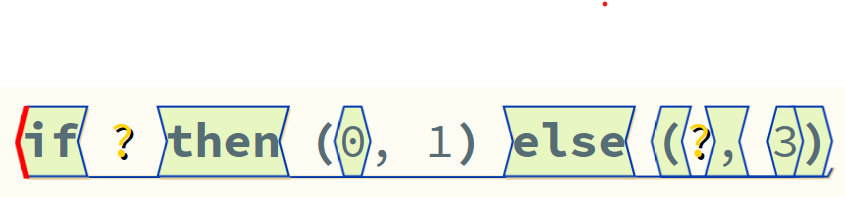
\includegraphics[width=0.5\textwidth]{Media/Figures/typejoin}
\caption{Type Slice Joins (note: Hazel syntax uses $\dyn$ also for expression holes)}
\label{fig:TypeJoins}
\end{figure}

This gets complex, requiring tracking all the data relating to which branches should be highlighted, and accumulating the inconsistent parts of failed joins for use in minimised error slices (demonstrated in \cref{sec:ErrorSlices}). I make use of custom OCaml let binding \cite{CustomLetOperators} to retain clarity while automatically combining branches in successful joins and combining inconsistencies in failed joins. For example, see \cref{fig:ArrowJoin}, where comments describe the logic abstracted by the custom bindings; note that all join-able type combinations use this same parallel binding logic to combine branches and inconsistencies.

\begin{figure}[h]
\small
\begin{minted}{reason}
...
| (Arrow(s1, s2), Arrow(s1', s2')) =>
      let+ s1j = join'(s1, s1') // If successful: binds the join to s1j and
                                // propagates the branch used joining s1, s1'
                                // Else: Propagates inconsistencies in s1, s1'
      and+ s2j = join'(s2, s2') // If both successful: binds the join to s2j and
                                // combines previously used branches joining s1, s2' 
                                // with those used joining s2 and s2'
                                // Else: propagates inconsistency in s1, s2' (if any)
                                // alongside new inconsistencies in s2, s2' (if any)
      and! branches_used = ();  // If both successful: Binds combined branches
                                // Else: propagates inconsistencies
      ( // If nothing failed, Returns the successful join.
        `SliceIncr((
          Slice(Arrow(s1_join, s2_join)), // The successful join
          choose_branch(branches_used, slice_incr1, slice_incr2),
        )) // Wrap with only one slice: the left if both branches used
        |> temp,
        branches_used, // combined branches used
      );
...
\end{minted}
\caption{Joining function types}
\label{fig:ArrowJoin}
\end{figure}

\subsection{Static Type Checking}\label{sec:TypeChecking}
Hazel is \textit{bidirectionally typed}, where the \textit{mode} (synthesis, analysis) is specified by the \code{Mode.t} type. Type checking calculates a type information object \code{Info.t} for each term, stored efficiently in a map from ID keys. \code{Info.t} is demonstrated in \cref{fig:Info} with arrows representing dependencies (e.g. a term's type depends on it's mode, self, typing context, and status).
\begin{figure}[h]
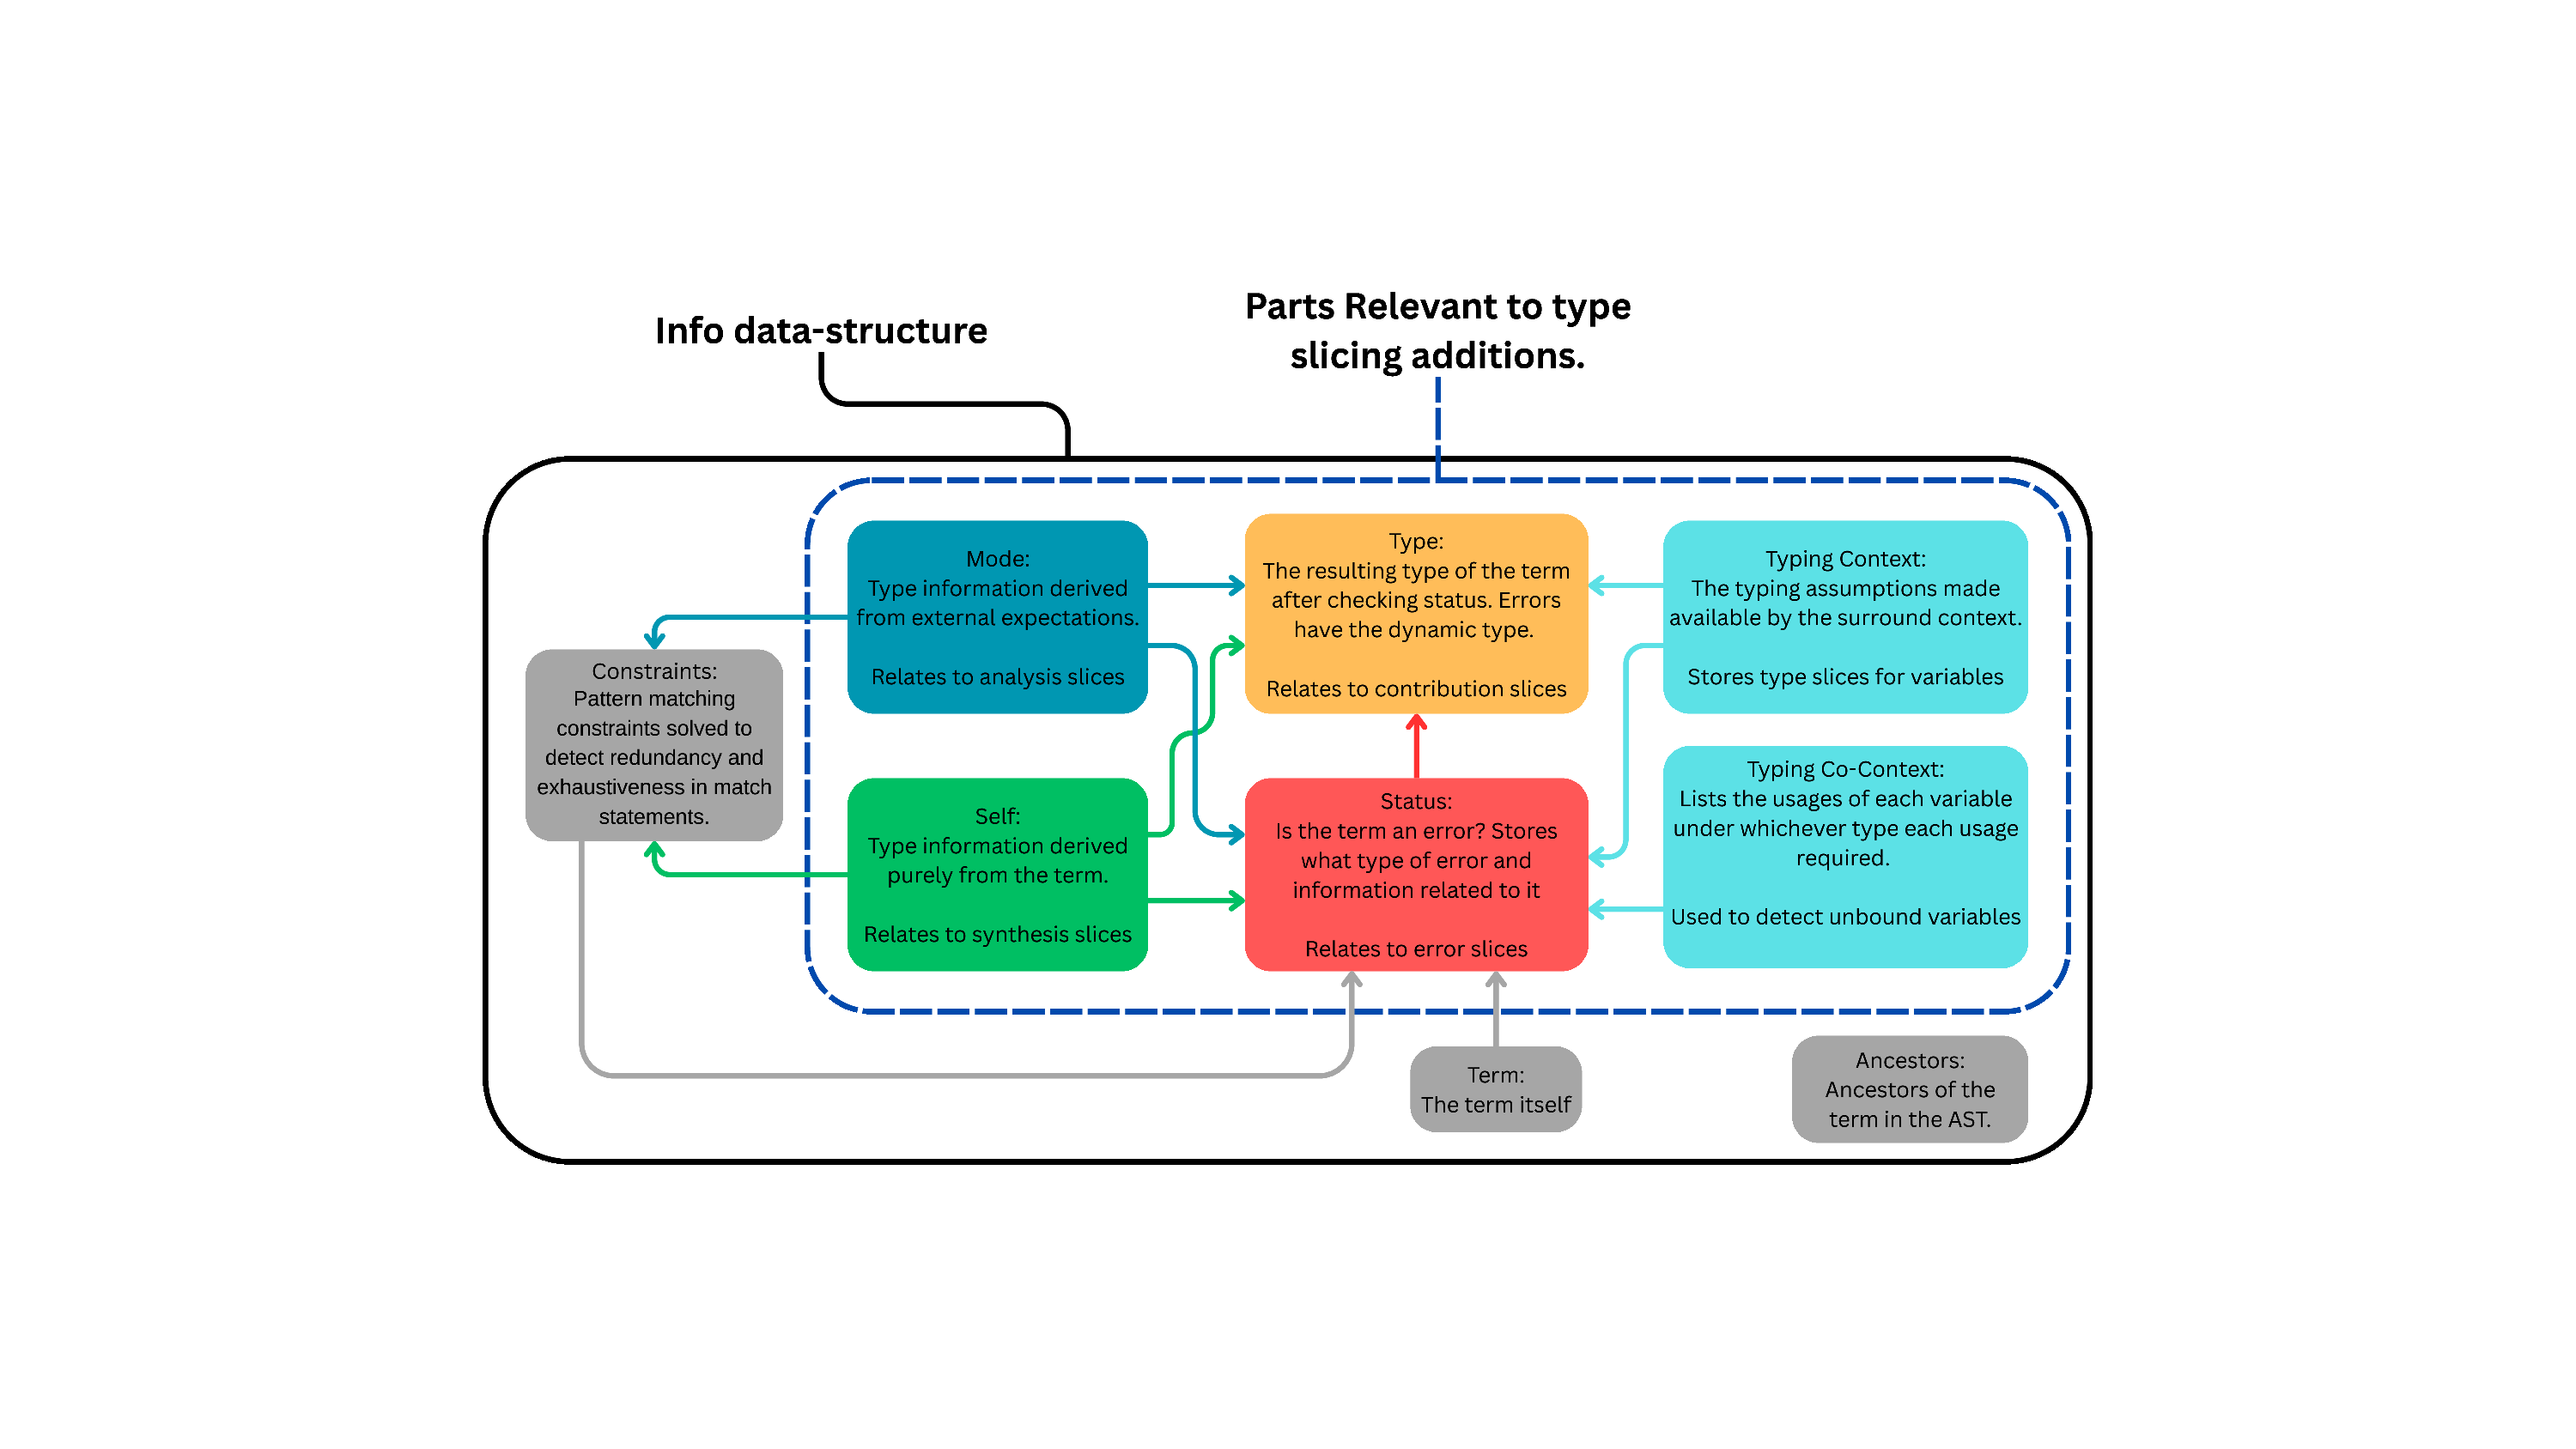
\includegraphics[width=1\textwidth, trim={8cm 5cm 8cm 5cm}, clip]{Media/Figures/info}
\caption{\code{Info.t} data-structure}
\label{fig:Info}
\end{figure}

\subsubsection{Self and Mode}
Slicing logic relating to synthesis slices and analysis slices is factored into \code{Self.t} and \code{Mode.t} respectively, cleanly segregated from the type checking code. Although, doing this still required full understanding of the type checker implementation, ensuring the correct IDs are sliced.

\subsubsection{Typing (Co-)Context}
The typing context and co-contexts are modified to use type slices. This deviates from the theoretical notion of an expression slice: the structural context in which the variable is used is untracked when passing through the context. Therefore, it requires using \textit{unstructured} code slices. It is useful in practice allowing slices calculated during binding to be retrieved usage, see \cref{fig:VarSlice}.
\begin{figure}[h]
\centering
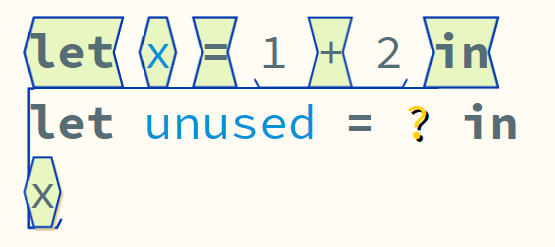
\includegraphics[width=0.3\textwidth]{Media/Figures/var_slice}
\caption{Type slice for variable \code{x}: includes it's binding and slice.}
\label{fig:VarSlice}
\end{figure}

\subsubsection{Status and Type}
The status, mode, and self are combined to determine a term's actual type, being dynamic if there is an error. When the expectations (mode, self) are inconsistent, the inconsistent slice information parts are tagged to the error status; \cref{sec:SlicingAnalysis} retrospectively considers what slice information to be extracted here. Additionally, contribution slices can extract the static parts of synthesis slices here. 

\subsection{Integration}
To support the full Hazel language, type slices needed to implement many functions, for example: type substitution, type normalisation, weak-head normalisation, tracking sum types, various structural matching functions etc. Additionally almost every usage of types in the codebase had to be refactored to use type slices (which are so easily pattern matched upon) while ensuring slices correctly maintained.

\subsection{User Interface \& Examples}
The type slices of the expression at the cursor (in red) are highlighted, see \cref{fig:SliceExamples}. Error slices distinguish between the synthesis and analysis parts with blue and red, see the evaluation examples \cref{sec:EvalExamples}.

\begin{figure}[h]
\centering
\begin{subfigure}[t]{0.45\textwidth}
\centering
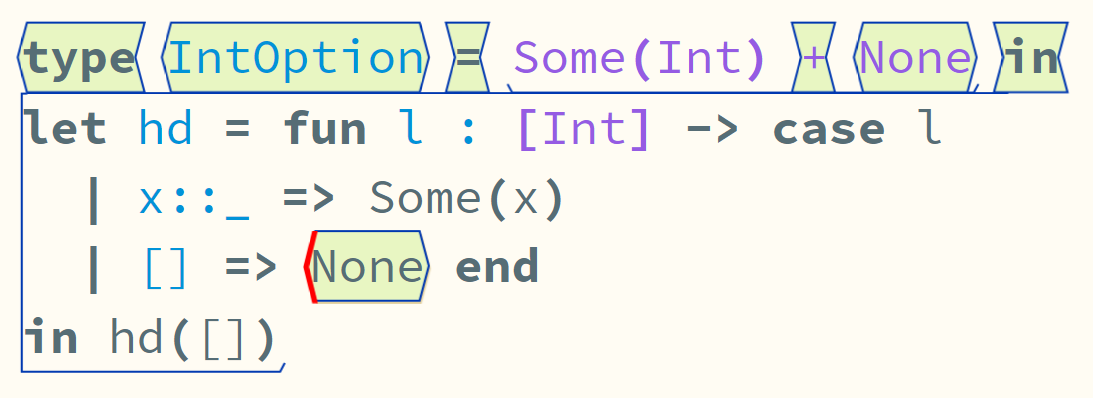
\includegraphics[width=1\textwidth]{Media/Figures/none_syn}
\caption{\code{None} synthesises \code{IntOption} due to it's type definition.}
\end{subfigure}$\qquad$
\begin{subfigure}[t]{0.45\textwidth}
\centering
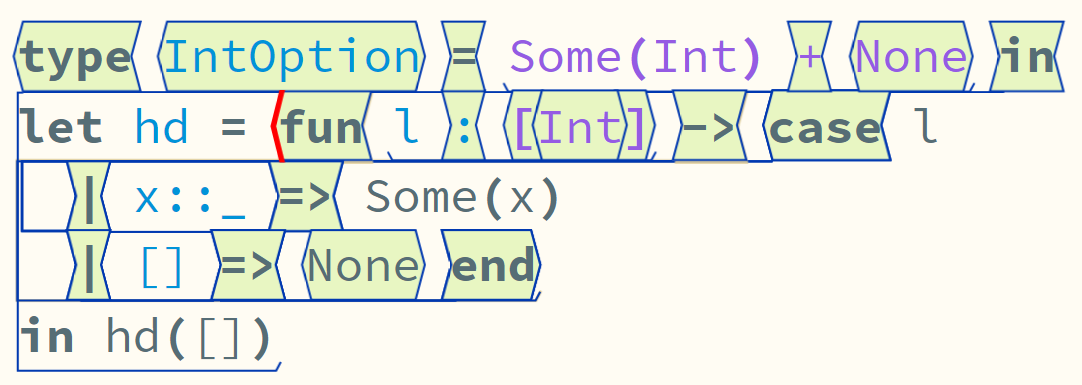
\includegraphics[width=1\textwidth]{Media/Figures/fun_syn}
\caption{The function synthesises \code{[Int]}$\to$ \code{IntOption} due to it's \code{[Int]} annotation and that the match branches synthesis \code{IntOption}. Both branches provide the same type information, only one branch (the last) is highlighted.}
\end{subfigure}
\begin{subfigure}[t]{0.45\textwidth}
\centering
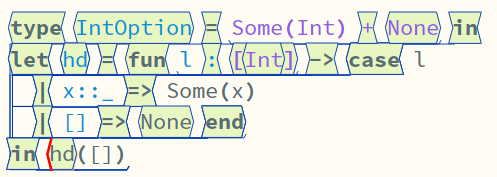
\includegraphics[width=1\textwidth]{Media/Figures/hd_syn}
\caption{The variable usage of \code{hd} synthesises \code{[Int]}$\to$ \code{IntOption} similarly, whose slice is retrieved from the typing context.}
\end{subfigure}$\qquad$
\begin{subfigure}[t]{0.45\textwidth}
\centering
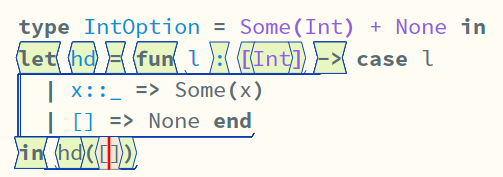
\includegraphics[width=1\textwidth]{Media/Figures/list_ana}
\caption{The list input is expected to be an \code{[Int]} as it is applied to \code{hd} which is a function annotated with input type \code{[Int]}.}
\end{subfigure}
\caption{Type Slices}
\label{fig:SliceExamples}
\end{figure}

\section{Cast Slicing Implementation}\label{sec:CastSlicingImplementation}
To implement cast slicing, replace casts between \textit{types} by casts between \textit{type slices}. Type slices are already type-indexed and retain all type information so can be used equivalently.

\subsection{Elaboration}\label{sec:Elaboration}
Cast insertion recursively traverses the unelaborated term, inserting casts to the term's statically determined type as stored in the \code{Info} data-structure. For example, a list literal recursively elaborate it's terms and joins their slices, casting to the join. Ensuring all the type slice information is retained and/or reconstructed during elaboration was a meticulous and error-prone process.

\subsection{Cast Transitions}
\Cref{sec:HazelDynamics} gave an intuitive overview of how casts are treated at runtime. Type-indexed slices allows cast slices to be decomposed in exactly the same way. 

However, as Hazel only checks consistency between casts between \textit{ground types}, there are two rules where new\footnote{As opposed to being derived from decomposition.} casts are \textit{inserted} (ITGround, ITExpand). The new types are created via a \textit{ground matching} relation taking the topmost compound constructor of types, e.g. ground functions \cref{fig:GroundFunction}. Relevant portions of the appendix are \cref{fig:groundtypes}, \cref{fig:instructions}, \cref{fig:groundmatch}.

As we store type slices incrementally, the part of the slice corresponding \textit{only} to the outer type constructor is the outer slice tag.

\begin{figure}
\[\tau_1 \to \tau_2 \match{\text{ground}} \dyn \to \dyn\]
\caption{Ground Matching Functions}
\label{fig:GroundFunction}
\end{figure}

\subsection{Unboxing}
When we know a final form's (\cref{sec:HazelFinalForms}) type, we may need to extract parts of the term according to the type during evaluation. For example, extracting the elements of a tuple. But due to casts and holes, this is not trivial \cite{LivePatternMatching}.

Slicing does not concern unboxing, but indeterminate evaluation (\cref{sec:IndetEval}) unveiled bugs within which had to be fixed. I raised and fixed these, eventually being merged into the main branch. \Cref{sec:UnboxingBugs} details this, after covering the required context on the unboxing implementation.

\subsection{User Interface \& Examples}
Type slices within casts can be selected from the evaluation result and displayed. This require reworking some of the dependencies of Hazel's model-view-update architecture to make sure the cursor has access to the code editor cell when inside the evaluation result cell.
\begin{figure}[h]
\centering
\begin{subfigure}{0.45\textwidth}
\centering
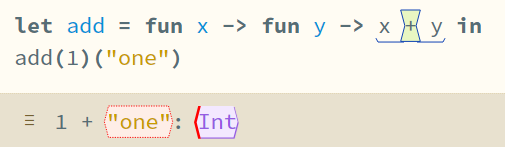
\includegraphics[width=1\textwidth]{Media/Figures/simple_cast_error}
\caption{A simple cast error blaming the plus operator for requiring the integer cast.}
\end{subfigure}
\begin{subfigure}{0.45\textwidth}
\centering
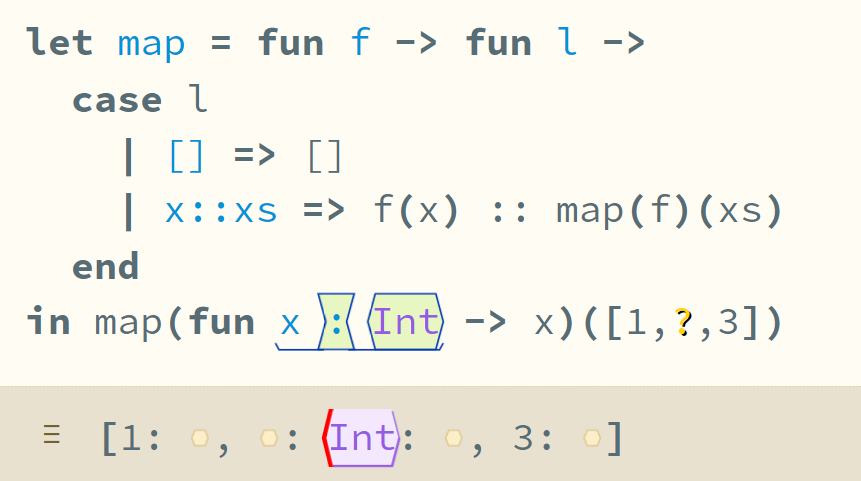
\includegraphics[width=1\textwidth]{Media/Figures/map_cast}
\caption{A hole cast to \code{Int} due to a mapped function annotated with an \code{Int} input.}
\end{subfigure}
\begin{subfigure}{0.65\textwidth}
\centering
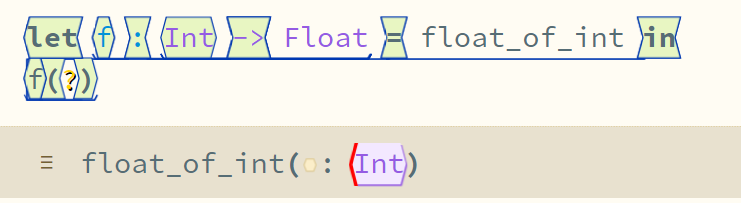
\includegraphics[width=1\textwidth]{Media/Figures/decompose_casts}
\caption{A decomposed cast. The input of the function takes only slice for the argument part \code{Int} of the function type $\code{Int} \to \code{Float}$.}
\end{subfigure}
\caption{Cast Slicing Examples}
\end{figure}
\section{Indeterminate Evaluation}\label{sec:IndetEval}
Dynamic errors include evaluation traces, which can aid in debugging \cite{TraceVisualisation}, yet static type errors lack such traces. Seidel et al. \cite{SearchProc} offer an algorithm  to search for these traces for static errors in OCaml by lazily, non-deterministically narrowing input holes to least specific values based on their usage context. 

This section creates a framework for non-deterministic evaluation of indeterminate expressions by lazily performing hole substitutions using type information from dynamic casts. Unlike Seidel, this supports more language features (all of Hazel), any number of inputs (holes), and exhaustive generation of these inputs. It is a general evaluation method, not limited to cast error searches. Specifics relating to cast errors and implementing search orderings, are covered in \cref{sec:SearchProcedure}.

\subsection{Resolving Non-determinism}
\label{sec:ResolvingNondeterminism}
To model infinite non-determinism I create a monadic DSL with an explicitly tree/forest-based representation. The forest model allows for varying low level search traversals. The module type of combinators is in \code{Nondeterminism.Search}; it's underlying parametric type is \code{t('a)} with \code{'a} being the type of the solutions. \Cref{sec:SearchMethods} discusses the actual implementations of this interface, giving four searching procedures.


In addition the functions from \Cref{sec:Nondeterminism}, I add standard \code{map} and \code{join} functions, and various other functions, e.g. \code{ifte} modelled after Mercury's if-then-else construct \cite{Mercury}.

\subsubsection{Abstracting Search Order: Forest Model}
Typical stream-based models of non-determinism \cite{ListOfSuccess} only admit the possibility of depth-first search (DFS). Stream concatenation provides no way of remembering choice points and backtracking before finishing a computation. 

Instead, we can use a model based on forests (lists of trees) \cite{Bunches}. Choice, similarly to streams, is performed by concatenating forests. Finally, to build tree structures, a \code{wrap} combinator wraps every tree up into a single tree with a new root, see \cref{fig:Wrap}. Effectively, this encodes a  notion of cost for search paths.

\begin{figure}[h]
\centering
\begin{subfigure}{0.45\textwidth}
\centering
\[\left[\ 1\quad ; \quad 2 \quad ; \quad 3\ \right]\]
\caption{\code{let x = return(1) <||>} \code{return(2)} \code{         <||> return(3)}}
\end{subfigure}
\begin{subfigure}{0.45\textwidth}
\centering
\[\left[\vcenter{\hbox{\begin{forest}
[$\cdot$ [4] [5]]
\end{forest}}}\right]\]
\caption{\code{let y = wrap(return(4) <||> return(5))}}
\end{subfigure}
\begin{subfigure}{0.45\textwidth}
\centering
\[\left[\vcenter{\hbox{\begin{forest}[$\cdot$ [1] [2] [3]]\end{forest}}} \quad ; \quad\vcenter{\hbox{\begin{forest}[$\cdot$ [4] [5]]\end{forest}}}\right]\]
\caption{\code{let z = wrap(x) <||> y}}
\end{subfigure}
\begin{subfigure}{0.45\textwidth}
\centering
\[\left[\vcenter{\hbox{\begin{forest}[$\cdot$ [$\cdot$ [1] [2] [3]][$\cdot$ [4] [5]]]\end{forest}}}\right]\]
\caption{\code{wrap(z)}}
\end{subfigure}
\caption{Forests Defined Using \code{wrap}}
\label{fig:Wrap}
\end{figure}

The DSL is extended with a \code{wrap : t('a) => t('a)} combinator. As \code{wrap} is abstract, the underlying implementation does not actually need to use a forest data structure. Therefore, DFS can still be efficiently implemented using regular streams. Finally, a \code{run} function produces a lazy list of solutions with ordering specified by the search method; these can be cycled through with some arrows in the UI.

\subsubsection{Recursive Functions}
As OCaml is strict, defining infinite choices via recursion can lead to non-termination during definition. I define a shorthand lazy application function \code{apply(f, x)} by \code{return(x) >>= f}, represented infix by \code{|>-}. Provided that bind lazily applies \code{f}, recursive functions can be written directly resulting in infinite choices without OCaml's strictness leading to infinite recursion.

\subsection{A Non-Deterministic Evaluation Algorithm}
\label{sec:IndetEvalAlgorithm}
This section demonstrates one indeterminate evaluation algorithm evaluating terms to concrete values in \cref{fig:IndetEvalBlock} with an accompanying code extract \cref{fig:IndetEval}.

\begin{figure}[h]
\centering
\scalebox{0.8}{\begin{tikzpicture}[
  node distance=1cm and 2cm,
  every node/.style={font=\small},
  startstop/.style={rectangle, rounded corners, draw, minimum width=3.5cm, minimum height=1cm, text centered, fill=blue!10},
  process/.style={rectangle, draw, minimum width=3.5cm, minimum height=1cm, text centered, fill=orange!20},
  decision/.style={diamond, draw, aspect=2, text centered, inner sep=1pt, fill=yellow!20},
  arrow/.style={-Latex}
]

% Nodes
\node (start) [startstop, draw=red] {Bind input to $d$};

\node (classify) [process, below=of start] {\texttt{take\_step}(d)};

\node (isValue) [decision, left=of classify] {Final value?};
\node (isIndet) [decision, below=of classify] {Indeterminate?};
\node (isStep) [decision, below right=of classify] {Can step?};

\node (retVal) [startstop, below=of isValue] {Return $d$ as result};

\node (instantiate) [process, below=of isIndet] {\texttt{instantiate}(d)};

\node (inst1) [process, left= of instantiate] {Instantiation 1};
\node (inst2) [process, below=of inst1] {Instantiation 2};
\node (instN) [below=of inst2] {$\vdots$};

\node (evalNext) [process, below=of isStep] {Step to $d'$};

\node (fail) [startstop, right=of classify] {Exception: \texttt{fail}};

% Arrows
\draw [arrow] (start) -- (classify);

\draw [arrow] (classify) -- (isValue);
\draw [arrow] (classify) -- (isIndet);
\draw [arrow] (classify) -- (isStep);
\draw [arrow] (classify) -- (fail);

\draw [arrow] (isValue) -- node[right] {Yes} (retVal);
\draw [arrow] (isIndet) -- node[right] {Yes} (instantiate);
\draw [arrow] (isStep) -- node[right] {Yes} (evalNext);

% Recursive loop from evalNext to start
\draw [arrow] (evalNext.south) |- ++(4,-1) |- (start.east);

% Instantiate forks
\draw [arrow] (instantiate.west) |- (inst1.east);
\draw [arrow] (instantiate.south) |- (inst2.east);
\draw [arrow] (instantiate.south) |- (instN.east);

% Loop back from each instantiation to start
\draw [arrow] (inst1.west) -- ++(-1,0) |- (start.west);
\draw [arrow] (inst2.west) -- ++(-1,0) |- (start.west);
\draw [arrow] (instN.west) -| ($(inst2.west)+(-1,0)$) |- (start.west);
\end{tikzpicture}}
\caption{Block diagram of indeterminate evaluation to values}
\label{fig:IndetEvalBlock}
\end{figure}

Instantiation is implemented by a \textit{non-deterministic} function \code{instantiate}, discussed in detail in \cref{sec:HoleInstantiation}: \[\code{Instantiation.instantiate : Exp.t => S.t(Exp.t)}\]

Evaluation steps are performed by a (deterministic) function \code{take_step}, classifing it's input as either (concrete) values, indeterminate values, steppable expressions. The step evaluator re-uses the Hazel stepper logic, which had existing bugs to be fixed: causing non-termination of fixed points\footnote{Due to incorrect management of closures; the main branch stepper is still broken as of May 9th.} and misclassifying concrete values as indeterminate values: 
\[\code{OneStepEvaluator.take_step : Exp.t => TryStep.t}\] 

To ensure that the search tree has finite branching factor, possibly infinite choices must be wrapped, e.g. evaluation steps. The actual implementation additionally threads state tracking number of instantiations and trace length throughout the algorithm.

\begin{figure}[h]
\small
\begin{minted}{reason}
module Make = (S: Search) => {
  module Instantiation = Instantiation.Make(S);
  open S;
  open S.Infix;
  
  let rec values = (d: DHExp.t) : S.t(DHExp.t) => {
    let step = OneStepEvaluator.take_step(d);
    switch (step) {
    | BoxedValue => return(d)
    | Indet => 
      d |>- Instantiation.instantiate
        >>= values;
    | Step(d') => wrap(d' |>- values);
    | exception (EvaluatorError.Exception(_)) => fail
    };
  };
};
\end{minted}
\caption{Indeterminate Evaluation to Values}
\label{fig:IndetEval}
\end{figure} 

The generalised indeterminate evaluation takes a higher-order \code{logic} function which determines the return logic (e.g. returning only results with cast errors).

\subsection{Hole Instantiation \& Substitution}\label{sec:HoleInstantiation}
This section details the semantics of hole instantiations, including Hazel-specific issues.

\subsubsection{Choosing which Hole to Instantiate}
\label{sec:ChooseHole}
An indeterminate term may contain \textit{multiple} holes or even \textit{no} holes. Which hole needs to be instantiated in order to \textit{make progress}?

When attempting to evaluate the indeterminate term some transitions rules require a sub-term to be concrete (e.g. a function during application). We chose to instantiate the hole that blocks the \textit{first} blocked transition rule. If latter holes were instantiated, the term might \textit{still} be unevaluable due to this first hole.

This is implemented using Hazel's evaluator abstraction (\code{EV_MODE}), which (rather obscurely\footnote{Lacking documentations and using advanced custom let operators \cite{CustomLetOperators}. Understanding took considerable time.}) separates this logic from the transition semantics. Therefore, hole choosing logic will automatically update to future changes in the transition semantics.

\subsubsection{Synthesising Terms for Types}
Suppose we know which hole to instantiate and to which type (\cref{sec:TypesForHoles}). How do we refine these holes fairly and lazily, to the \textit{least specific} value that allows evaluation to continue?

Base types must be instantiated directly to their (possibly infinite set of) values, for example:
\paragraph{Booleans} \code{return(true) <||> return(false)}.
\paragraph{Integers} A recursive definition using lazy application \code{|>-}, see \cref{fig:Integers}:
\begin{figure}[h]
\begin{minted}{reason}
let rec ints_from = n => return(n) <||> wrap(n + 1 |>- ints_from)
let nats = ints_from(0)
let negs = ints_from(1) >>| n => -n
let ints = nats <||> wrap(negs) 
\end{minted}
\begin{subfigure}{0.45\textwidth}
\centering
\scalebox{0.8}{$\left[\ n \quad ; \quad \vcenter{\hbox{\begin{forest}
[$\cdot$ [$n+1$] [$\cdot$ [$n + 2$] [$\cdot$ [$n+3$] [...]]]]
\end{forest}}}\right]$}
\caption{\code{ints_from(n)}}
\end{subfigure}
\begin{subfigure}{0.45\textwidth}
\centering
\scalebox{0.8}{$\left[\ 0 \quad ; \quad \vcenter{\hbox{\begin{forest}
[$\cdot$ [$1$] [$\cdot$ [$2$] [$\cdot$ [$3$] [...]]]]
\end{forest}}} \quad ; \quad \vcenter{\hbox{\begin{forest}
[$\cdot$ [$-1$] [$\cdot$ [$-2$] [$\cdot$ [$-3$] [...]]]]
\end{forest}}}\right]$}
\caption{\code{ints}}
\end{subfigure}
\caption{Enumerating Integers}
\label{fig:Integers}
\end{figure}
 
\paragraph{Strings} A string is either \textit{empty} or is a string with a first character from a finite set. We can recursively wrap all strings, prefixed by each character. See \cref{fig:Strings}:
\begin{figure}[h]
\begin{minted}{reason}
let chars = ... // Choice every single letter string to be considered
let rec strings = () => return("") 
  <||> wrap(chars >>= chr => 
            (() |>- strings) >>= str => 
            chr ++ str)) 
\end{minted}
\caption{Enumerating Strings}
\label{fig:Strings}
\end{figure}
\

Other types are \textit{inductive}, these can be represented indirectly by lazily instantiating only their \textit{outermost} constructors: 
 
\paragraph{Lists} A list is either the empty list, $[\ ]$ or a cons $\dyn_1 :: \dyn_2$. To retain the correct dynamic type information, $\dyn_2$ must be cast back to the list type. 
\paragraph{Sum Types} Enumerate each of the sum's constructors with their least specific value.
\paragraph{Functions} Constant functions have least specific values $\lambda \_.\ \dyn$. The function may then be applied to any value, and it's result synthesised after application. This can synthesise any return value, hence errors in the usage of the function will be detected. But, if the \textit{input} has an erroneous type but is not yet caught due to partial annotations, these will be lost. This is rare, and could be mitigated by generating the identity function where possible.

\paragraph{Maintaining Correct Casts}
Holes have a dynamic type at runtime. Therefore, the hole's context \textit{expects} a dynamic expression. Therefore, we must cast every instantiation back to the dynamic type.

\subsubsection{Substituting Holes}\label{sec:HoleSubstitutionImplementation}
Holes can be bound to variables in the execution environment, and may also be duplicated, before they are required to be instantiated, see \cref{fig:HoleDuplication}. Every occurrence must be substituted.

Hole substitution was described as part of the Hazel calculus \cref{sec:HoleSubstitution}. But, unexpectedly, the main Hazel branch does not yet implement it. A full implementation of metavariables and delayed closures is complex. Therefore, as hole closures are not required for hole instantiation,\footnote{Instantiations do not contain variable references.} I use existing term ids identify holes, ensuring these are maintained and propagated correctly, so that duplicated holes retain the same ID.\footnote{All of elaboration and dynamics required these checks.}

Substitutions must also be performed within closures, eagerly evaluating the results to ensure that closures bind variables to values. 

\subsection{Determining the Types for Hole Substitutions}
\label{sec:TypesForHoles}
If we know which hole to instantiate, how do we know which type to instantiate it to? This logic is highly specific to Hazel's cast semantics, with many Hazel-specific issues arising.

For efficiency, my implementation both determines \textit{which hole}, and it's \textit{type information} during the same pass.

\paragraph{Directly from Casts}
Most of the time, a hole is directly surrounded by a cast, whose type information can be used to perform an instantiation.

\paragraph{Cast Laziness}\label{sec:CastLaziness}
However, this is \textit{not} always the case. For efficiency reasons, Hazel treats casts over compound data lazily, e.g. casts around tuples will only by pushed inside upon usage of a component of the tuple. Treating casts eagerly is a significant change to the Hazel semantics, so was opted against. \Cref{sec:EvalCastLaziness} evaluates the consequence of this choice.

\begin{figure}
\centering
\begin{minipage}{.45\textwidth}
\centering
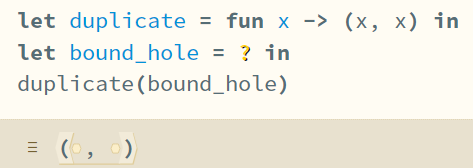
\includegraphics[width=0.8\linewidth]{Media/Figures/duplicate_hole}
\caption{Duplicated Holes}
\label{fig:HoleDuplication}
\end{minipage}%
\begin{minipage}{.45\textwidth}
  \centering
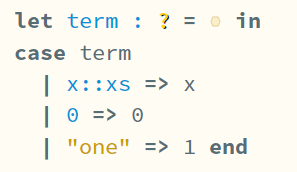
\includegraphics[width=0.5\linewidth]{Media/Figures/dynmatch}
\caption{Dynamic/Type-case Match Statement}
\label{fig:DynamicPatternMatching}
\end{minipage}
\end{figure}

\paragraph{Pattern Matching}
\label{sec:PatternMatching}
Does a hole even have only one possible type? Dynamic pattern matching actually allows terms to be matched against \textit{non-uniform} types. See \cref{fig:DynamicPatternMatching}, having patterns of multiple types. Hence instantiating to any of the types might allow progress.

We can collect each of these possible types from the elaborated casts inserted on the \textit{branches}, non-deterministically rewrapping them around the scrutinee.
\ 
\par
\ 
\par
\subsubsection{Extended Match Expression Instantiation (Pattern Instantiation)}
\label{sec:ExtendedPatternMatching}
An interesting extension was partially implemented which improves code coverage and additionally detects errors within patterns. It instantiates holes in a match expression according also to the \textit{structure} of each pattern, allowing the instantiation to prioritise searching along each branch. We instantiate the scrutinee with the least specific versions which match the patterns on each branch, e.g. \dyn\code{::}\dyn\ for \code{x::xs}. However, difficulties come when the scrutinee is a compound term, or when least specific matches only indeterminately matching earlier branches. Further details addressing these issues can be found in \cref{sec:extendedmatching}.

\section{Search Procedure}\label{sec:SearchProcedure}
Now that an framework for indeterminate evaluation has been specified, the DSL implementations and cast error search logic can be addressed. The search procedure can be switched on via a toggle in the settings.

\subsection{Detecting Relevant Cast Errors}
\label{sec:CastFailureDetection}
To search for cast errors, we must first define what one is. A reasonable definition is terms which contain \textit{cast failures}; in Hazel, these are casts between \textit{inconsistent ground types}. However, this has some issues:

\paragraph{Multiple Cast Failures} Terms may have multiple cast failures, some of which discovered during static type checking and inserted via elaboration. But these failures won't stop evaluation until necessary. Therefore, we should consider only the casts which are directly \textit{causing} a term to get stuck, this is implemented similarly to choosing which hole to instantiate (\cref{sec:ChooseHole}).

\paragraph{Cast Laziness}
\label{sec:SearchCastLaziness}
Only casts between \textit{ground} types are checked for consistency. Due to cast laziness (\cref{sec:CastLaziness}), some compound terms will be cast between inconsistent types, but \textit{not} placed within a \textit{cast failure}. As before, this issue is ignored due to requiring large changes to Hazel semantics, the evaluation finds it to be a rare occurrence.

\paragraph{Dynamic Match Statements} When matching dynamically on values with different types, the instantiations wrap the scrutinee in casts to each type. If any of these casts failed, they should not count as witnesses, as they were introduced entirely by the instantiation procedure. 

\subsection{Searching Methods}\label{sec:SearchMethods}
I implement \textit{four} different search methods, implementing the non-determinism signature specified in \cref{sec:ResolvingNondeterminism}.

\paragraph{Depth First Search (DFS)}
Modelling DFS by streams is a typical method \cite{ListOfSuccess}: implementing choice and conjunction via appending, and \code{wrap} being identity function (no internal tree structure needed).

\paragraph{Breadth First Search (BFS)}
Breadth first search represents forests by sequences of sequences \cite{BFSCombinators}, with the $n$th inner sequences representing every solution in the $n$th level of the trees in the forest. Then, \code{choice} concatenates each level, and \code{wrap} conses the empty list, pushing every solution one level down.

The other monadic operators are complex, but \code{join : t(t('a)) => t('a)} can be visualised  in \cref{fig:BFSJoin}: for simplicity showing joining trees of trees, which is extended to forests by choicing the trees in each inner forest.

\begin{figure}[h]
\centering
\[\vcenter{\hbox{\begin{subfigure}{0.45\textwidth}
\centering
\scalebox{1}{\begin{tikzpicture}[scale=0.8, transform shape,
  main tree/.style={grow=right, sibling distance=3cm, level distance=3cm},
  sub tree/.style={grow=right, sibling distance=1cm, level distance=1cm},
  every node/.style={circle, draw, minimum size=6mm, inner sep=0pt},
  main node/.style={draw=red, thick},
  sub node/.style={draw=blue, fill=blue},
  invisible/.style={draw=blue}
  ]

% Main tree in x–z plane
\begin{scope}[canvas is xz plane at y=0, main tree]
% Level 1 rectangle
    \fill[cyan!40, fill opacity=0.5, rounded corners] (2.5,-2.8) rectangle (3.5,2.8);
    % Level 2 rectangle
    \fill[green!40, fill opacity=0.5,  rounded corners] (5.5,-4) rectangle (6.5,1);
\node[main node] (root) {}
  child {node[main node] (a) {}
    child {node[main node] (a1) {}}
    child {node[main node] (a2) {}}
  }
  child {node[main node] (b) {}
  };
\end{scope}

% Subtrees with rectangles directly inside

% Depth 3 subtrees
\foreach \n in {root} {
  \begin{scope}[shift={(\n)}, canvas is yz plane at x=0, sub tree]
    % Level 1 rectangle
    \fill[cyan!40, fill opacity=0.5, rounded corners] (0.4,-1.2) rectangle (1.5,1.2);
    % Level 2 rectangle
    \fill[green!40, fill opacity=0.5,  rounded corners] (1.5,-0.6) rectangle (2.6,1.6);
    
    \node[invisible] {}
      child {node[sub node] {}}
      child {node[invisible] {}
        child {node[sub node] {}}
        child {node[sub node] {}}
      };
  \end{scope}
}

% Depth 2 subtrees
\foreach \n in {a, b} {
  \begin{scope}[shift={(\n)}, canvas is yz plane at x=0, sub tree]
    % Level 1 rectangle
    \fill[green!40, fill opacity=0.5, rounded corners] (0.4,-1.2) rectangle (1.6,1.2);
    
    \node[invisible] {}
      child {node[sub node] {}}
      child {node[sub node] {}};
  \end{scope}
}

\foreach \n in {a1, a2} {
  \begin{scope}[shift={(\n)}, canvas is yz plane at x=0, sub tree]
    \node[sub node] {};
  \end{scope}
}

\end{tikzpicture}}
\caption{Before Join: Singleton forest of singleton forests (list of lists of lists of lists). Rectangles are the inner lists of the forests.}
\end{subfigure}}}
\quad\mapsto\quad
\vcenter{\hbox{\begin{subfigure}{0.45\textwidth}
\scalebox{1}{\begin{tikzpicture}[scale=0.8, transform shape,
  main tree/.style={grow=right, sibling distance=3cm, level distance=3cm},
  level 2/.style={sibling distance=1cm},
  sub tree/.style={grow=right, sibling distance=1cm, level distance=2cm},
  every node/.style={circle, draw, minimum size=6mm, inner sep=0pt},
  main node/.style={draw=red, thick},
  sub node/.style={draw=blue, fill=blue},
  invisible/.style={draw=blue}
  ]

% Main tree in x–z plane
\begin{scope}[canvas is xz plane at y=0, main tree]
% Level 1 rectangle
    \fill[cyan!40, fill opacity=0.5, rounded corners] (2.5,-5.4) rectangle (3.5,5.4);
    % Level 2 rectangle
    \fill[green!40, fill opacity=0.5,  rounded corners] (5.5,-7) rectangle (6.5,6);
\node[main node] (root) {}
  child {node[main node] (a) {}
    child {node[sub node] (a1) {}}
    child {node[sub node] (a3) {}}
    child {node[sub node] (a2) {}}
    child {node[sub node] (a4) {}}
  }
  child {node[sub node] (c) {}
  }
  child {node[invisible] (d) {}
    child {node[sub node] (d1) {}}
    child {node[sub node] (d2) {}}
  }
  child {node[main node] (b) {}
    child {node[sub node] (b1) {}}
    child {node[sub node] (b2) {}}
  };
\end{scope}
\end{tikzpicture}}
\caption{After Join: Flattened into a single forest (list of lists) by rotating vertical trees into horizontal plane. Solid circles are the solutions actually stored in the BFS lists.}
\end{subfigure}}}
\]
\caption{BFS Join}
\label{fig:BFSJoin}
\end{figure}
This join and mapping can be defined lazily; the standard definition for \code{bind} from the paper \cite{Bunches} does not work easily in OCaml due to its strictness.

\paragraph{Bounded Depth First Search (BDFS)}
BFS is fair, avoiding non-termination (for finite branching factor), but it has \textit{exponential} space complexity in the depth of the level being explored \cite{NorvigAI}. In comparison, DFS only requires space linear in the depth explored.

Bounded DFS, performs successive depth-bounded depth first searches, retaining low space complexity of DFS while avoiding unfairness. Previous solutions are repeatedly explored, but this does not increase the already exponential time complexity of the search.

Spivey \cite{Bunches} represent this by functions \code{Int => ['a, Int]}, calculating solutions within an integer depth bound. Solutions are tagged with their remaining depth budgets, which allows keeping only the fringe solutions (zero budget) upon each iteration, so the same solution will not appear twice.

I augment this into an \code{Bound.t => (Bool, ['a, Bound.t])}, implemented as a functor allowing customised depth bound increases. The boolean is false only if no search path reaches the depth bound, in which case the trees have been fully searched and the algorithm can be terminated.


\paragraph{Interleaved Streams (IDFS)}
Streams, but with choice and conjunction via interleaving also ensures fairness. This works even for trees with infinite branching factor. However, interleaving has a linear space complexity, resulting in exponential space complexity as with BFS.

\section{Repository Overview}
\paragraph{Branches}
The submitted code contains the three most important branches of this project (\texttt{Evaluation}, \texttt{witnesses-type-slicing}, \texttt{contribution-slices}). The \texttt{Evaluation} branch factors out a \code{Js_of_ocaml} \cite{JSOO} dependency from the Hazel core library, meaning evaluation code can be run natively and on the command line; however, the web interface is therefore unusable on this branch.

\paragraph{Hazel Architecture}
The Hazel architecture demonstrates in \cref{fig:Architecture} with green files/directories added, orange files modified \textit{significantly}, and blue files modified \textit{insignificantly} (but still needing to know how they work) or unmodified. 97 files were added/edited, not all can fit, so anything omitted is considered insignificant to understanding this project.
 \Cref{fig:Evaluation} shows the structure of the evaluation modules.
\begin{figure}[h]
 \tiny
 \centering
 \scalebox{0.93}{\begin{tabular}{llp{7cm}}
 Dir & Description\\
 {\color{Green}\texttt{data/*}} & \multicolumn{2}{l}{Program corpus, pre-filtering}\\
 {\color{Green}\texttt{results/*}} & \multicolumn{2}{l}{Results}\\
 {\color{Green}\ \ \ \ \  $\vdash$}&{\color{Green}\texttt{./benchmarks.file}} & Results of search procedure benchmarks\\
 {\color{Green}\ \ \ \ \  $\vdash$}&{\color{Green}\texttt{./results.file}} & Results of effectiveness analysis\\
 {\color{Green}\ \ \ \ \  $\vdash$}&{\color{Green}\texttt{./failure\_classification.txt}} & Classification of failed searches in BDFS\\
 {\color{Green}\ \ \ \ \  $\vdash$}&{\color{Green}\texttt{./log.file}} & Log from which results are derived\\
 {\color{Green}\texttt{ParseData.ml}} & \multicolumn{2}{l}{Evaluation string data loaded into \texttt{.ml} file}\\
 {\color{Green}\texttt{CastSliceUtil.ml}} & \multicolumn{2}{l}{Cast slice size calculation and errors classification}\\
 {\color{Green}\texttt{SlicingUtil.ml}} & \multicolumn{2}{l}{Type slice size calculation and errors classification}\\
 {\color{Green}\texttt{ResourceLimits.ml}} & \multicolumn{2}{l}{Unix alarm-based evaluation timeout}\\
 {\color{Green}\texttt{Settings.ml}} & \multicolumn{2}{l}{Ctx to type check \& evaluate under}\\
 {\color{Green}\texttt{Util.ml}} & \multicolumn{2}{l}{Maths utilities}\\
 {\color{Green}\texttt{CastSliceUtil.ml}} & \multicolumn{2}{l}{Cast slice size calculation and errors classification}\\
 {\color{Green}\texttt{Results.ml}} & \multicolumn{2}{l}{Calculates results log}\\
 \end{tabular}}
 \caption{Evaluation Data, Results, and Modules}
 \label{fig:Evaluation}
\end{figure}
\begin{figure}
 \centering
 \tiny
 \scalebox{0.93}{\begin{tabular}{lllllp{4cm}}
 Dir & Description\\
 {\color{orange}\texttt{src/*}} & \multicolumn{5}{l}{Hazel source code}\\
 {\color{orange}\ \ \ $\vdash$}&{\color{orange}\texttt{./haz3lcore/*}} & \multicolumn{4}{l}{Core semantics library}\\
 & {\color{orange}\ \ \ \ \ \ \ \ $\vdash$} & {\color{orange}\texttt{./dynamics/*}} & \multicolumn{3}{l}{Hazel dynamics}\\
 & & {\color{Green}\ \ \ \ \ \ \ \ $\vdash$} & {\color{Green}\texttt{./indeteval/*}} & \multicolumn{2}{l}{Indeterminate Evaluation}\\
 & & & {\color{Green}\ \ \ \  \ \ \ \ $\vdash$} & {\color{Green}\texttt{./Nondeterminism.re}} & Non-determinism DSL \& implementations\\
 & & & {\color{Green}\ \ \ \  \ \ \ \ $\vdash$} & {\color{Green}\texttt{./Searching.re}} & Collection of default search procedures\\
 & & & {\color{Green}\ \ \ \  \ \ \ \ $\vdash$} & {\color{Green}\texttt{./RedexHoleType.re}} & Chooses hole to instantiate and its possible types\\
 & & & {\color{Green}\ \ \ \  \ \ \ \ $\vdash$} & {\color{Green}\texttt{./CastErrorChecker.re}} & \\
 & & & {\color{Green}\ \ \ \  \ \ \ \ $\vdash$} & {\color{Green}\texttt{./OneStepEvaluator.re}} & \\
 & & & {\color{Green}\ \ \ \  \ \ \ \ $\vdash$} & {\color{Green}\texttt{./Instantiation.re}} & {\raggedright Instantiation Logic \& Hole Substitution}\\
 & & & {\color{Green}\ \ \ \  \ \ \ \ $\vdash$} & {\color{Green}\texttt{./IndetEvaluation.re}} & Generic indeterminate evaluation algorithm\\
 & & {\color{Green}\ \ \ \ \ \ \ \ $\vdash$} & {\color{Green}\texttt{./state/*}} & {\color{Green}\texttt{./IndetEvaluatorState.re}} & {\raggedright IndetEval State}\\
 & & {\color{orange}\ \ \ \ \ \ \ \ $\vdash$} & {\color{orange}\texttt{./stepper/*}} & \multicolumn{2}{l}{Hazel stepper (Bug fixes required)}\\
 & & {\color{blue}\ \ \ \ \ \ \ \ $\vdash$} & {\color{blue}\texttt{./evaluator.re}} & \multicolumn{2}{l}{Big-step semantics: evaluator stack machine}\\
 & & {\color{orange}\ \ \ \ \ \ \ \ $\vdash$} & {\color{orange}\texttt{./transition/*}} & \multicolumn{2}{l}{Transition semantics \& Unboxing}\\
 & & & {\color{orange}\ \ \ \  \ \ \ \ $\vdash$} & {\color{orange}\texttt{./Casts.re}} & Cast calculus: modified sum type semantics\\
 & & & {\color{blue}\ \ \ \  \ \ \ \ $\vdash$} & {\color{blue}\texttt{./PatternMatch.re}} & Pattern matching\\
 & & & {\color{blue}\ \ \ \  \ \ \ \ $\vdash$} & {\color{blue}\texttt{./Transition.re}} & Small-step semantics\\
 & & & {\color{orange}\ \ \ \  \ \ \ \ $\vdash$} & {\color{orange}\texttt{./Unboxing.re}} & Unboxing: Various bug fixes\\
 & {\color{orange}\ \ \ \ \ \ \ \ $\vdash$} & {\color{orange}\texttt{./lang/term/*}} & \multicolumn{3}{l}{Hazel AST definitions \& fundamental functions}\\
 & & {\color{orange}\ \ \ \ \ \ \ \ $\vdash$} & {\color{orange}\texttt{./Grammar.re}} & \multicolumn{2}{l}{Adds type slices; replace types with slices}\\
 & & {\color{blue}\ \ \ \ \ \ \ \ $\vdash$} & {\color{blue}\texttt{./IdTagged.re}} & \multicolumn{2}{l}{ID tagging terms}\\
 & & {\color{Green}\ \ \ \ \ \ \ \ $\vdash$} & {\color{Green}\texttt{./TypSlice.re}} & \multicolumn{2}{l}{Type Slices (and its utility function)}\\
 & & {\color{blue}\ \ \ \ \ \ \ \ $\vdash$} & {\color{blue}\texttt{./Exp.re}} & \multicolumn{2}{l}{Expressions}\\
 & & {\color{orange}\ \ \ \ \ \ \ \ $\vdash$} & {\color{orange}\texttt{./Typ.re}} & \multicolumn{2}{l}{Types: Added branch tracking logic for joins}\\
 & & {\color{blue}\ \ \ \ \ \ \ \ $\vdash$} & {\color{blue}\texttt{./Pat.re}} & \multicolumn{2}{l}{Patterns}\\
 & & {\color{blue}\ \ \ \ \ \ \ \ $\vdash$} & {\color{blue}\texttt{./TPat.re}} & \multicolumn{2}{l}{Type Patterns}\\
 & {\color{orange}\ \ \ \ \ \ \ \ $\vdash$} & {\color{blue}\texttt{./prog/*}} & \multicolumn{3}{l}{Settings \& Program results (now returning lists)}\\
 & {\color{orange}\ \ \ \ \ \ \ \ $\vdash$} & {\color{orange}\texttt{./statics/*}} & \multicolumn{3}{l}{Hazel statics}\\
 & & {\color{orange}\ \ \ \ \ \ \ \ $\vdash$} & {\color{orange}\scalebox{.8}{\texttt{./ConstructorMap.re}}} & \multicolumn{2}{l}{Sum constructors: Adds Constructor joining logic}\\
 & & {\color{blue}\ \ \ \ \ \ \ \ $\vdash$} & {\color{blue}\texttt{./Ctx.re}} & \multicolumn{2}{l}{Typing assumptions context}\\
 & & {\color{blue}\ \ \ \ \ \ \ \ $\vdash$} & {\color{blue}\texttt{./CoCtx.re}} & \multicolumn{2}{l}{Typing assumptions co-context}\\
 & & {\color{blue}\ \ \ \ \ \ \ \ $\vdash$} & {\color{blue}\texttt{./Coverage.re}} & \multicolumn{2}{l}{Pattern matching exhaustivity \& redundancy checks}\\
 & & {\color{orange}\ \ \ \ \ \ \ \ $\vdash$} & {\color{orange}\texttt{./Self.re}} & \multicolumn{2}{l}{Expectation independent type info: Synthesis slice logic}\\
 & & {\color{orange}\ \ \ \ \ \ \ \ $\vdash$} & {\color{orange}\texttt{./Mode.re}} & \multicolumn{2}{l}{Expectation based type info: Analysis slice logic}\\
 & & {\color{orange}\ \ \ \ \ \ \ \ $\vdash$} & {\color{orange}\texttt{./Info.re}} & \multicolumn{2}{l}{Statics information: Error slices}\\
 & & {\color{orange}\ \ \ \ \ \ \ \ $\vdash$} & {\color{orange}\texttt{./Statics.re}} & \multicolumn{2}{l}{Type Checker: Bindings slicing logic}\\
 & & {\color{orange}\ \ \ \ \ \ \ \ $\vdash$} & {\color{orange}\texttt{./Elaborator.re}} & \multicolumn{2}{l}{Elaboration: Casts are now between slices}\\
 & {\color{blue}\ \ \ \ \ \ \ \ $\vdash$} & {\color{blue}\texttt{./tiles/*}} & \multicolumn{3}{l}{Structure editor tiles}\\
 & {\color{blue}\ \ \ \ \ \ \ \ $\vdash$} & {\color{blue}\texttt{./zipper/*}} & \multicolumn{3}{l}{Structure editor zipper and parser}\\
 & {\color{Green}\ \ \ \ \ \ \ \ $\vdash$} & {\color{Green}\texttt{./Joins.re}} & \multicolumn{3}{l}{Slice joins utilities}\\
 {\color{blue}\ \ \ $\vdash$}&{\color{blue}\texttt{./haz3lmenhrir/*}} & \multicolumn{4}{l}{LR(1) Parser}\\
 {\color{orange}\ \ \ $\vdash$}&{\color{orange}\texttt{./haz3lweb/*}} & \multicolumn{4}{l}{MVU Web Interface: see \texttt{docs/ui-architecture.md}}\\
&{\color{orange}\ \ \ \ \ \ \ \  $\vdash$} & {\color{orange}\texttt{./app}} & {\color{orange}\texttt{./editors/*}} & \multicolumn{2}{l}{Threads cursor into \texttt{./result/*} editors}\\
& & &{\color{orange}\ \ \ \ \ \ \ $\vdash$} & {\color{orange}\texttt{./decoration/Deco.re}} & {Adds UI for slices and error slices}\\
&{\color{orange}\ \ \ \ \ \ \ \  $\vdash$} & {\color{orange}\texttt{./Settings.re}} & \multicolumn{3}{l}{Adds indet eval and search settings}\\
&{\color{orange}\ \ \ \ \ \ \ \  $\vdash$} & {\color{orange}\texttt{./www/*}} & \multicolumn{3}{l}{\texttt{.css} files: Adds slice colourings}\\
&{\color{orange}\ \ \ \ \ \ \ \  $\vdash$} & {\color{orange}\texttt{./util/*}} & {\color{orange}\scalebox{.8}{\texttt{./WorkerServer.re}}} & \multicolumn{2}{l}{Live evaluator: Now uses BDFS indet eval.}\\
 {\color{blue}\ \ \ $\vdash$}&{\color{blue}\texttt{./pretty/*}} & \multicolumn{4}{l}{Formatting for Hazel code}\\
 {\color{blue}\ \ \ $\vdash$}&{\color{blue}\texttt{./util/*}} & \multicolumn{4}{l}{Utility modules (adds \code{Base.Sequence})}\\
{\color{orange}\texttt{test/*}} & \multicolumn{5}{l}{Test cases: Updates to use type slices}\\
{\color{Green}\ \ \ $\vdash$} & {\color{Green}\texttt{./Test\_Unboxing.re}} & \multicolumn{4}{l}{Adds list unboxing tests (also merged into \code{dev} branch) }
 \end{tabular}}\ 
 \vspace{12pt}
 
\textbf{Key:} {\color{Green} Additions}, {\color{orange} Significant Modifications}, {\color{blue} Insignificant or No Modifications}
 \caption{Hazel Architecture \& Additions}
 \label{fig:Architecture}
\end{figure}


